\chapter{Grundlagen}

\printmyminitoc{1}

In diesem Kapitel werden die Grundlagen für die Arbeit erläutert.
Dabei wird sich auf die wichtigen Begriffe und Technologien für den Rahmen dieser Arbeit fokussiert.
Damit wird ein Verständnis für die Arbeit geschaffen und die Grundlage für die weiteren Kapitel gelegt.

\section{CAN-Bus}
Bei einem CAN-Bus handelt es sich um eine serielle Netzwerktechnologie, 
die mehrere Geräte mit einem Kabel verbindet.
Die Entwicklung des CAN-Bus wurde von Bosch im Jahr 1983 begonnen \cite[Seiten 2--10]{Voss2008}. 
Im Jahr 1986 wurde der erste CAN-Bus Standard 
veröffentlicht.
Die Motivation der Entwicklung war die effiziente Kommunikation zwischen den Steuergeräten in einem Auto. 
Als günstigen
Seiteneffekt konnte damit die Kabelmenge reduziert werden, da alle Geräte mit einem Bus verbunden werden können.
Durch die höhere Zuverlässigkeit und Funktionalität des CAN-Bus, wurde dieser schnell in der Autoindustrie etabliert.
Aber auch in anderen Sektoren, wie z. B. der Medizintechnik, der Gebäudeautomation oder der Luftfahrt, spielt der
CAN-Bus mittlwerweile eine wichtige Rolle.
\\
Man sprich von einem Bussystem, da mehrere Geräte miteinander über diesen miteinander verbunden werden \cite[Seiten 13--19]{Voss2008}. 
Die Geräte auf an dem Bus sind in dem Fall die Knoten. Alle sind gleichberechtigt und können Nachrichten senden und empfangen.
Die Nachrichten werden nach Broadcasting-Prinzip übertragen. Dabei wird jede Nachricht von allen Knoten empfangen, 
aber nur die Knoten, welche die Nachricht benötigen, verarbeiten sie. \\
Die Nachrichten werden nicht explizit bestätigt, da dies zu einer größeren unnötigen Last auf dem Bus führen würde.
Trotzdem erwartet der Sender eine positive Bestätigung der Nachricht. Das Passiert mit einem Acknowledge (ACK) Bit 
im CAN-Frame, wie in Abbildung \ref{fig:canframe} zu sehen ist. Wenn eine Nachricht nicht bestätigt wird, 
sendet der Sender eine Fehlermeldung auf den Bus. Wenn ein Sender zu viele fehlerhafte Nachrichten sendet, soll
dieser sich selbst logisch von dem CAN-Bus trennen. Eine Nachricht wird als fehlerhaft angesehen, wenn z. B. die Prüfsumme
nicht stimmt oder die Nachricht nicht dem Standard entspricht.

\begin{figure}[H]
    \centering
    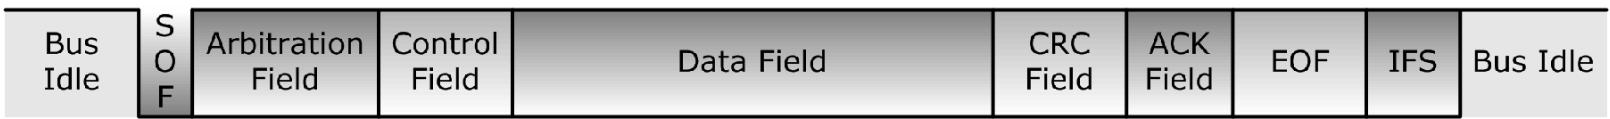
\includegraphics[scale=0.25]{images/canFrame.png}
    \caption{Aufbau eines CAN-Frames \cite{Voss2008}}
    \label{fig:canframe}
\end{figure}

Die auf den Bus gesendeten Daten werden mit einer Nachrichten-ID
versehen, welche die Priorität der Nachricht angibt. Die Priorität existiert, damit zeitkritische Nachrichten
schneller verarbeitet werden können.Die Nachrichten mit der niedrigsten ID haben die höchste Priorität.
Die Maximale Länge einer Nachricht beträgt 8 Byte. 
Auf dem CAN-Bus kann eine maximale Baudrate von \ 1Mbit/s erreicht werden.
Zusätzlich kann durch die geringe Länge der Nachrichten geringe Latenz erreicht werden. 
Insgesamt ist der CAN-Bus damit gut für Echtzeitanwendungen geeignet, da die Reaktionszeit der Knoten möglichst gering gehalten wird.
\\
Alle Knoten in einem CAN-Bus sind mit einem zweiadrigen Kabel verbunden \cite[Seite 132]{Voss2008}. 
Diese werden als High (CAN\_H) und Low (CAN\_L) 
bezeichnet. Der Bus ist an beiden Enden mit einem Widerstand von 120 $\Omega$ abgeschlossen, um Reflexionen zu vermeiden.
\\
Eine Nachricht auf einem CAN-Bus ist in einem CAN-Frame verpackt \cite[Seite 36]{Voss2008}. 
Der Aufbau eines CAN-Frames ist in Abbildung \ref{fig:canframe} zu sehen.
Dieser beginnt mit einem Startbit, welches Start of Frame (SOF) genannt wird. Darauf folgt das Arbitration Field, 
in dem die Nachrichten-ID und ein Bit RTR (Remote Transmission Request) gesetzt wird. Das RTR-Bit wird gesetzt,
wenn der Sender eine Antwort auf die Nachricht erwartet. Das Control Field wird für die Datengröße und die Nachrichtenlänge
verwendet. Im Data Field sind die eigentlichen Nutzdaten kodiert. Das CRC Field enthält eine Prüfsumme, welches die Richtigkeit
der Nachricht überprüft. Hier folgt ein ACK Field, welches die Prüfsumme bestätigt. Die Nachricht endet mit einem End of Frame (EOF).
Danacht folgt ein Interframe Space (IFS) von 3 Bit, welches eine Pause zwischen den Nachrichten darstellt.

\subsection{J1939-Protokoll}
Das Standard CAN-Protokoll hat einen 11 Bit Identifier, während das erweiterte CAN-Protokoll 29 Bit Identifier
besitzt \cite{Murvay2018}. Dabei gibt es mehrere Standards, die den erweiterten Identifier verwenden.
Der relevante Standard für diese Arbeit ist der SAE J1939-Protokoll.
Die Society of Automotive Engineers (SAE) hat das J1939-Protokoll entwickelt, um die Kommunikation in Nutzfahrzeugen
zu verbessern. Der Fokus liegt auf der Kommunikation mit dem Antrieb des Fahrzeugs. Der 11-Bit-Identifier wird in J1939 
auf 29 Bit erweitert, um eine größere Anzahl verschiedener Nachrichten zu ermöglichen.\\
Auf einem CAN-Bus können der Standard 11 Bit Identifier und der erweiterte 29 Bit Identifier gleichzeitig verwendet werden.
Eine Nachricht mit dem 11 Bit Identifier wird bevorzugt vor einer Nachricht mit 29 Bit Identifier, wenn diese die gleiche
Priorität haben. Die spezifierten Baudraten sind hier 250 kbit/s und 500 kbit/s. 
\begin{figure}[H]
    \centering
    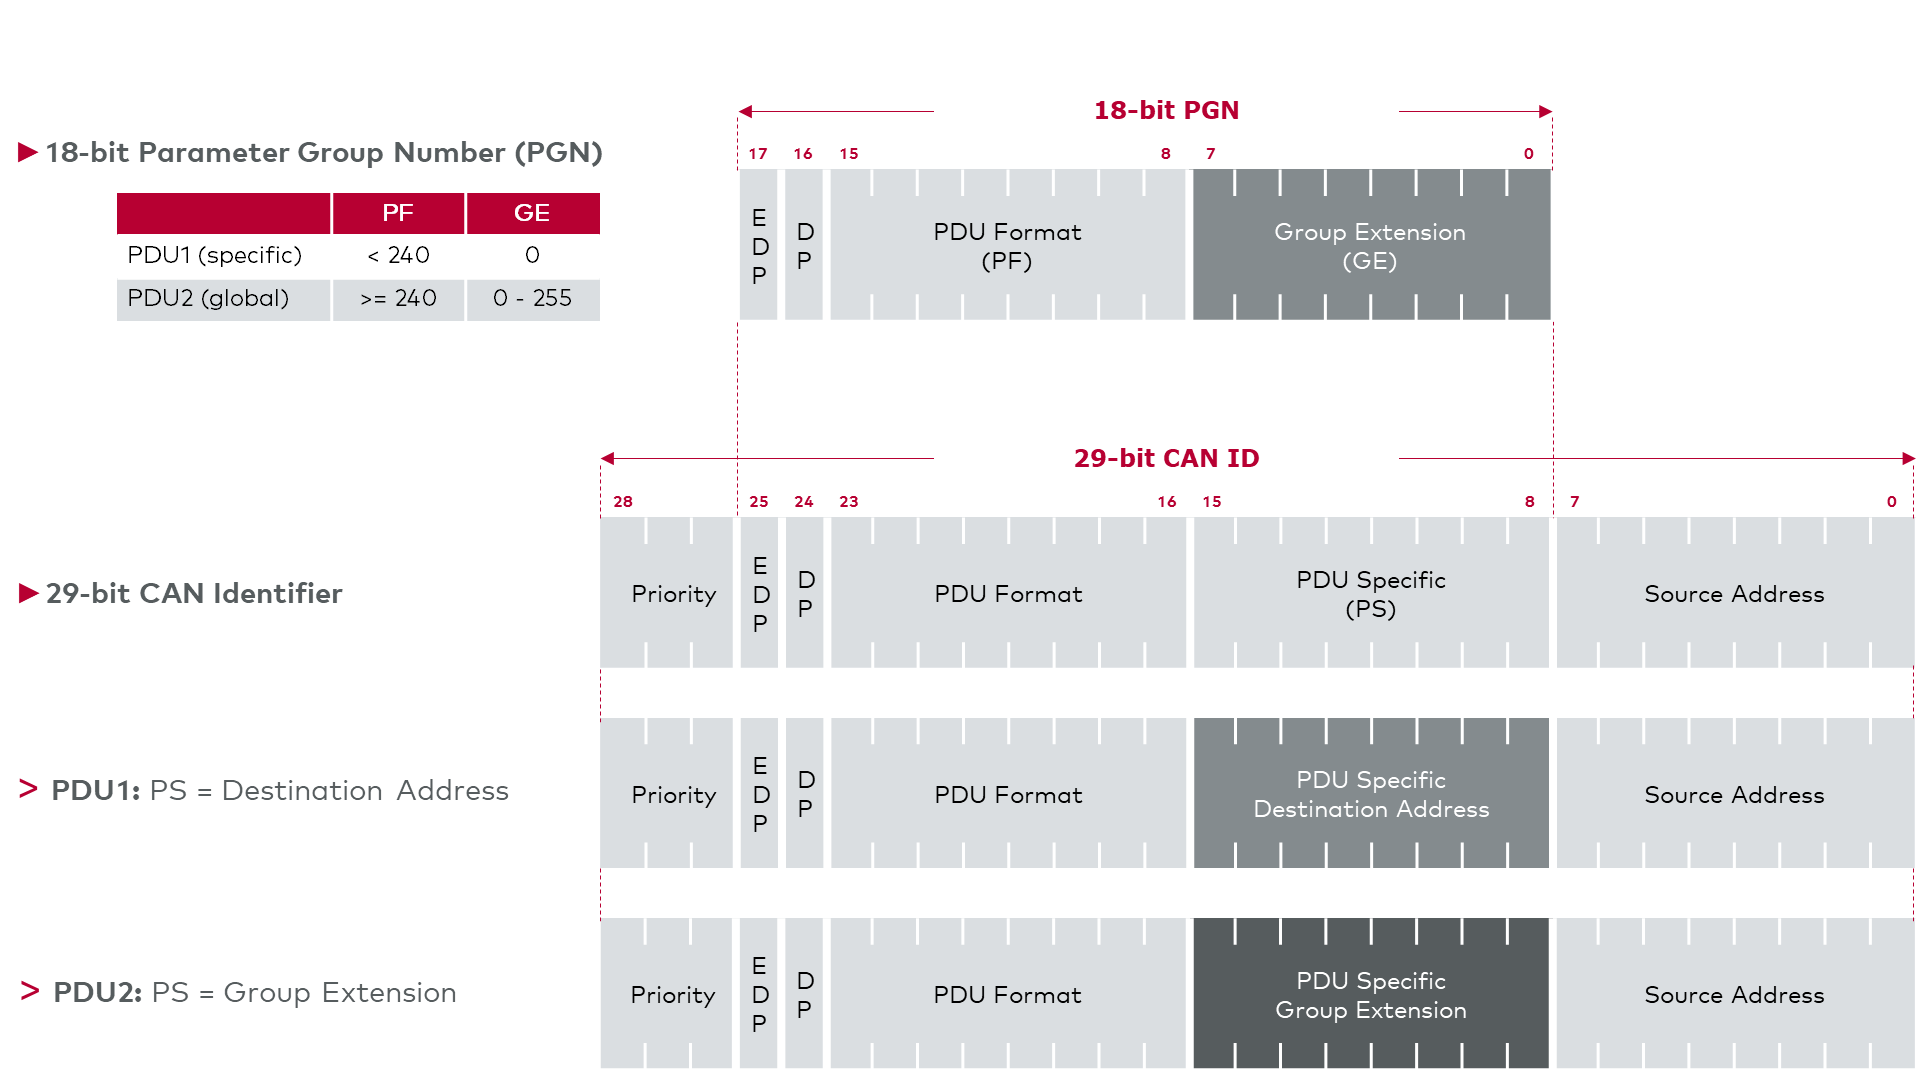
\includegraphics[scale=0.28]{images/j1939header.png}
    \caption{Header einer J1939-Nachricht auf dem CAN-Bus \cite{VectorSAE}}
    \label{fig:j1939header}
\end{figure}
In Abbildung \ref{fig:j1939header} ist der 29 Bit Identifier einer J1939-Nachricht zu sehen.
Die Hauptkomponenten des erweiterten Identifier sind die Priority, eine Parameter Group Number (PGN) und eine Quell-Adresse.
Das PGN-Feld ist aus 1 Bit Data Page (DP), 1 Bit Extended Data Page (EDP), einer Protocol Data Unit (PDU) und einem PDU spezifischen 
Feld (PS) aufgebaut. Die DP und EDP bestimmen mit welchem Standard die 
Nachricht gesendet wird. Für SAE J1939 werden aber nur drei Kombinationen verwendet \cite{VectorSAE}.
Das PS-Feld kann entweder eine Zieladresse oder eine Gruppenerweiterung (GE) sein. Welches PS-Feld
verwendet wird, hängt von der PDU ab. Wenn diese einen Wert von unter 240 hat, wird das PS-Feld als Zieladresse verwendet. 
In dem anderen Fall wird das PS-Feld als Gruppenerweiterung verwendet. \\
Trotz des Broadcasting-Prinzips soll nicht jede Nachricht von jedem Knoten verarbeitet werden \cite{Murvay2018}.
Die Zieladresse ermöglicht es, dass eine Nachricht nur von dem designierten Knoten verarbeitet wird.
Um eine Nachricht an alle Knoten 
zu senden, wird die Zieladresse auf 255 gesetzt. Mit der Gruppenerweiterung ist es nicht möglich eine Nachricht 
zielgerichtet an bestimmte Geräte zu senden. 

\section{NMEA-0183}
NMEA-0183 ist ein Standard für die Kommunikation zwischen verschiedenen Geräten in der Schifffahrt \cite{nmea0183}. Es handelt sich um
einen Schnittstellenstandar, der von der National Marine Electronics Association (NMEA) entwickelt wurde. 
Er kann nur einen Sender haben, aber mehrere Empfänger. Die Daten werden in ASCII-Format übertragen. In den Daten 
können unter anderem Informationen über die Position, die Geschwindigkeit und die Richtung des Schiffes enthalten sein.

\section{Raspberry Pi} \label{sec:raspberrypi}
Ein Raspberry Pi ist ein Einplatinencomputer, der von der Raspberry Pi Foundation entwickelt wurde. 
Dieser hat den Prozessor mit Grafikeinheit, Arbeitsspeicher, Speicher und Anschlüssen auf einem einzigen Board integriert.
Es handelt sich um einen vollwertiger Computer, der kleiner als normale PCs ist. Zusätzlich kann dieser mit einem normalen Betriebssystem
betrieben werden. Aus diesem Grund wurd der Raspberry Pi im Rahmen dieser Arbeit verwendet.
Trotzdem gibt es ein spezielles Betriebssystem, das für den Raspberry Pi entwickelt wurde, das Raspberry Pi OS (ehemals Raspbian).
Dieses basiert auf der Linux-Distribution Debian. Um viele Funktionen erfüllen zu können, hat der Raspberry Pi viele Anschlüsse.
Der Raspberry Pi 5 hat 4 USB-Anschlüsse, 2 Micro-HDMI-Anschlüsse, 1 Ethernet-Anschluss, 1 USB-C-Anschluss 
für die Stromversorgung und einen Micro-SD-Kartensteckplatz.